% ----------------------------------------------------------
% Apêndices
% Documentos gerados pelo próprio autor
% ----------------------------------------------------------

% ---
% Inicia os apêndices
% ---
\begin{apendicesenv}
	
	% Imprime uma página indicando o início dos apêndices
	\partapendices
	
	% ----------------------------------------------------------
	\chapter{Proposta Inicial}
	% ----------------------------------------------------------
	
	Esse apêndice trás a proposta inicial apresentada pela equipe. 
	
	\section{Ideia}
	
	O nosso Projeto Integrador tem como ideia uma rede social para pais de crianças atípicas. No intuito de desenvolver um aplicativo, temos a visão de construir funcionalidades que tragam informações, trocas de experiências, desenvolvimento de um perfil de acordo com o interesse do usuário, recomendações de lugares oportunos para seus filhos e realização de notificações que passam a integrar mais os pais como a nossa aplicação. 
	
	Sendo assim, passando por cada funcionalidade podemos destacar cada elas como: 
	
	
	
	
	
	\section{Feed de notícias:}
	Essa função terá como propósito informar os pais a respeito de como lidar quando temos filhos atípicos, quais são as característica que diferencia seus filhos, os tipos de crianças e adolescentes que podemos encontrar, assim como textos publicados na internet de educadores e profissionais da saúde que são especializados no assunto, sendo constantemente atualizados. 
	
	\section{Fórum:}
	Essa funcionalidade tem como o principal objetivo a troca de experiência. Vamos construir salas de conversa de texto divididos por categorias como: Saúde, Educação, Alimentação e Lazer. A partir dessas categorias, o utilizador conseguirá criar subcategorias e assim poder compartilhar informações, dúvidas e debates a respeito do seu interesse.
	
	Os fórum também serão organizados de forma que os mais relevantes fiquem em destaques. Serve também para as postagens em destaques, podendo ser curtidas e fixadas em cada categoria. 
	
	\section{Perfil:}
	Nesse local, basicamente, o usuário irá poder compartilhar informações sobre si mesmo e os seus interesses e até mesmo compartilhar a sua história e experiências na descrição do seu perfil. Assim, será possível maior identificação de outros usuários com o perfil descrito, podendo ter mais interações e conhecimentos a respeito de cada um dentro da nossa rede social. 
	
	\section{Comunicação Instantânea: }
	Nessa parte, temos a ideia que o usuário possa enviar e receber mensagens. Assim, essa comunicação mais privada pode estabelecer que informações sejam compartilhadas e resolvidas com mais velocidades. 
	
	\section{Localização: }
	No intuito de manter uma maior interação entre os usuários e compartilhamento de informações, a possibilidade de compartilhar a localização dentro do aplicativo serve para encontrar pessoas que possam ter crianças que possuem o mesmo tipo de  necessidades especiais e que estão próximas uma das outras, além disso será permitido compartilhar também locais que recebam ou são projetadas para crianças e adolescentes portadoras de deficiência como forma de recomendações para outros pais. 
	
	\section{Notificações: }
	Nessa interação, o nosso aplicativo conseguirá fornecer mensagens que exibirá fora da UI do app para fornecer comunicados dos fóruns ou de mensagens privadas, além de outras informações oportunas como informações do feed de notícias. Dessa maneira, os usuários poderão tocar na notificação para abrir seu app e executar uma ação diretamente da notificação. 
	
	
	% ----------------------------------------------------------
	
	\section{Objetivo}
	Sabendo que a inclusão de crianças portadoras de alguma deficiência é um desafio para a sociedade e que mesmo amparadas por lei, elas possuem ainda grandes dificuldades de interagir no meio social. Essa dificuldade também é passada para seus familiares, pois são eles iniciam a infra-estrutura para que seus filhos possam ter uma qualidade de vida melhor. Entretanto, saber lidar com isso de primeira pode gerar frustrações e sentimentos de culpa, além de se sentirem perdidos para escolher escolas, médicos, fisioterapeutas, fonoaudiólogos, psicólogos para ajudar no desenvolvimento de suas crianças e adolescentes.  Dessa maneira, a ideia de criar um aplicativo focado nesse nicho de pessoas tem como objetivo criar uma rede online para que possam se sentir, cada vez mais, amparadas e incluídas dentro da sociedade. Esse recurso de acolhimento mesmo que de forma online é de grande eficiência, uma vez que ao existir contato com outros pais e crianças que passam pela mesma situação traz fortalecimento emocional, compartilhamento de cuidados em diferentes casos e recomendações de profissionais e ambientes que recebam pessoas portadoras de deficiência de maneira integrada com a sociedade.
	
	
	
	% ----------------------------------------------------------
	\section{Tecnologias}
	Segundo o relatório State of Mobile 2022, da empresa “data.ai” que utiliza Ciência de Dados para analisar o mercado mobile em todo o mundo, o Brasil é líder na utilização de smartphones. A população brasileira passa, em média, 5,4 horas diárias consumindo conteúdos pelo celular, enquanto a média global é de 4,8 horas. 
	
	Diante dessa massiva demanda por aplicativos móveis, é crescente a busca dessa indústria por soluções que abarquem diversas áreas da vida da população de forma simples e eficiente. Somente em 2021, foram lançados 2 milhões de aplicativos móveis, de acordo com o mesmo relatório da “data.ai”.
	
	Como resultado, hoje existem ferramentas open-source de alta qualidade que possibilitam a construção de aplicativos intuitivos, acessíveis e escaláveis, tornando a entrega de novas soluções mais rápidas e fáceis às equipes de software. 
	
	Então, dado o sucesso dos aplicativos, escolhemos construir nesse formato o (nome do app), pois enxergamos que poderemos utilizar de práticas e ferramentas bem estabelecidas no mercado e assim alcançar um número expressivo de usuários dentro de uma área aquecida e em expansão.
	
	O foco atual é a plataforma Android, amplamente utilizada no Brasil e que de acordo com relatório de 2020 Impacto econômico e social do Android no Brasil, da consultoria digital “Bain & Company”, é uma tecnologia que teve impacto decisivo para o acesso à internet de milhares de brasileiros. Contudo, dado o uso do React Native, esse aplicativo poderá ser facilmente expandido para iOS e Web.
	
	A fim de realizar a prototipação, a equipe utilizará a ferramenta Figma, editor colaborativo online de design gráfico que permite a criação de interfaces de alta fidelidade e que ajudará os desenvolvedores a construir telas coesas e baseadas nos conceitos e práticas de User Experience (UX) e User Interface (UI).
	
	Para a construção desse aplicativo, sabe-se que serão necessários serviços, processos, persistência dos dados e uma interface. Por conta disso, nós optamos pelo uso da Stack MERN, essa sigla se refere a um conjunto de tecnologias amplamente utilizado para o desenvolvimento de aplicações, sendo respectivamente a base de dados não relacional MongoDB, um módulo minimalista de roteamento chamado Express.js, um framework desenvolvido pelo Facebook baseado em React feito para o desenvolvimento de aplicativos mobile e multiplataforma que usa de recursos nativos das plataformas de smartphone que é o React Native e por fim o Node.js que é um executor de Javascript no lado do servidor para criação de aplicações que executam no servidor como APIs (Application Programming Interface, isto é interface de programação de aplicações).
	
	Nesse contexto, necessitamos provisionar, documentar e testar a aplicação desenvolvida. Para lidar com o ambiente em máquinas de diferentes sistemas operacionais utilizaremos os containers Docker para possuirmos alta descartabilidade e reprodutibilidade do ambiente de desenvolvimento. Da mesma forma, entende-se que a existência de uma API bem documentada é essencial para um desenvolvimento com menos ruído de informação, então utilizaremos a especificação OpenAPI, também conhecida como especificação Swagger para documentar os recursos da API. Enfim, com o objetivo de atingir alta confiabilidade também optamos pelo uso do Jest, um framework de testes que facilita o processo de execução, criação, manutenção, gera relatórios sobre a cobertura total de código e aponta trechos de código que carecem de testes.
	
	Junto disso, em questão de comunicação entre cliente e servidor, temos como escolha por requisições (HTTP) para comunicação síncrona e para comunicação em tempo real utilizaremos a tecnologia WebSockets. Como parte dessa comunicação, haverão integrações com o Firebase (plataforma desenvolvida pelo Google para a criação de aplicativos móveis e da Web) para autenticação social com o Google e uso de mapas do Google Mapas.
	Eventualmente, compreende-se que precisaremos disponibilizar esse aplicativo (app) ao usuário final e para isso pretendemos utilizar a plataforma PlayStore para publicação da versão Android do app, será utilizado a plataforma de nuvem Mongodb Atlas para implantar em produção o banco de dados e o Heroku para provisionar em produção a API.
	
	
	
	%---------------------------------------------------------------------------------------
	\section{Análise comparativa com outras aplicações}
	Como objeto de comparação foram selecionados três aplicativos já presentes no mercado, sendo dois deles aplicativos direcionados ao público do espectro autista, o Minha Rotina Especial e o TippyTalk, e o terceiro sendo uma das redes sociais mais utilizadas e famosas do mundo, o Facebook.
	Para que o comparativo seja melhor traçado, é interessante que os aplicativos escolhidos para o exercício sejam apresentados, e que, dentro de cada um, seja feita a comparação da aplicação com o ConnectTEA:
	
	\subsection{Minha Rotina Especial:}
	Baseado na metodologia do terapeuta ocupacional Régis Nepomuceno, criador do projeto, o aplicativo foi desenvolvido para auxiliar na organização e clareza de rotina para aqueles que necessitam de acompanhamento no dia a dia.
	Integra diferentes informações, consciente de que as atividades diárias são grandes oportunidades de aprendizado e desenvolvimento de várias habilidades.
	A ideia é que as atividades da rotina sejam vinculadas/relacionadas à imagens, áudios e relatórios que facilitem o entendimento da atividade e também para que profissionais possam fazer um melhor acompanhamento da criança.
	
	\subsection{Comparado com o Minha Rotina Especial:}
	O foco do Minha Rotina Especial é bem afunilado e específico, apoiar na organização das atividades da rotina, trazendo uma maior elucidação para a criança que necessita de apoio. Enquanto o ConnectTEA tem um foco mais amplo, que se expande para o âmbito de sociabilização, interação online e disseminação de informações, tudo isso através das funcionalidades já explicitadas antes. Resumidamente, são dois aplicativos com ideias diferentes para um mesmo público.
	
	
	\subsection{TippyTalk:}
	O aplicativo tem o intuito de facilitar a comunicação das pessoas que têm dificuldades devido a alguma deficiência verbal/social. O funcionamento dele se dá através da tradução de imagens para mensagens de texto, mensagens essas que podem ser enviadas a algum parente, pessoa próxima ou um outro celular.
	O cerne da ideia é que os pais ou responsáveis possam tirar fotos e descrevê-las da forma mais pessoal possível para a criança, de maneira que ela possa identificar todas as imagens sem complicação alguma.
	Além do texto também é possível fazer uma gravação de voz sobre as imagens, trazendo o recurso auditivo para dar maior apoio àquele que fará o uso do aplicativo.
	
	\subsection{Comparado com o TippyTalk:}
	O TippyTalk tem o único intuito de possibilitar uma comunicação mais simples durante a realização de tarefas do dia a dia, sejam elas dentro ou fora de casa; Já o ConnectTEA se estende para outras vertentes que não a comunicação rotineira, algumas das funcionalidades que exemplificam isso são o fórum, criado para debates extensos e de variados assuntos, o feed de notícias e o uso da localização do usuário, funcionalidade que possibilita a recomendação de locais próximos aos usuários que são recomendados por outros integrantes da plataforma.
	
	
	\subsection{Facebook:}
	Por definição dos seus três criadores, Mark Zuckerberg, Dustin Moskovitz e Chris Hughes, o Facebook tem como propósito configurar um espaço virtual no qual as pessoas possam encontrar umas às outras e interagir através postagens de texto e/ou fotos, possibilitando debates e acesso à diferentes pontos de vista, objetivando a criação de um mundo mais transparente.
	
	\subsection{Comparado com o Facebook:}
	O Facebook tem como o objetivo conectar pessoas através da comunicação por diferentes mídias que a plataforma suporta. O grande diferencial da ConnectTEA nessa comparação é que nela há um enfoque que não existe no Facebook, o apoio direto ao público do espectro autista e seus familiares/pessoas próximas, conectando-as com pessoas em situação semelhante através de funcionalidades análogas às presentes na rede social americana.
	
	
	
	
	
	%---------------------------------------------------------------------------------------
	\section{Possíveis Integrações}
	A partir de uma análise, foram constatados que algumas integrações com outras aplicações e API externas podem ser feitas. Levando em consideração que o projeto a ser desenvolvido é uma rede social, algumas partes vão ser feitas através de integrações para melhor experiência do usuário para compartilhamento de posts, login e visualização daquilo que lhe é pertinente. 
	
	\subsection{Login:}
	As ferramentas necessárias aqui são as principais de redes sociais de e-mails, caso o usuário não queira fazer o cadastro diretamente pela aplicação. 
	\subsection{Feed de notícias:}
	API de noticiais do governo e google news C
	\subsection{Comunicação Instantânea:}
	Chat bot pelo para FAQ, chat Pro. 
	\subsection{Localização:}
	Google maps
	\subsection{Compartilhamento:}
	Principais redes de conversa e sociais além do e-mail. 
	
	%---------------------------------------------------------------------------------------
	\section{Parcerias}
	Escolhemos parcerias para que mais pessoas possam saber da nossa rede social, indicar amigos que são, possuem filhos ou conhecem alguém no espectro de autismo.
	
	As parcerias além de ajudarem a divulgar a nossa rede social para inclusão e reconhecimento de pessoas nessa condição, também podem auxiliar para uma maior inserção na sociedade através de cursos com pessoas devidamente capacitadas.
	
	\subsection{Canal Autismo}
	Revista periódica especializada em transtorno do Espectro do Autismo (TEA)
	
	\subsection{Fundação Getúlio Vargas - FGV}
	Fundação de educação e pesquisa de grande excelência no Brasil
	
	\subsection{Generation Brasil}
	ONG mundial que qualifica alunos para estudarem programação.
	
	\subsection{Meios de comunicação online e impressos}
	Meios de comunicação impressos trazem mais credibilidade e solidez.
	
	\subsection{Influenciadores}
	Influenciadores diversos, especialmente os que possuem algum espectro autista. 
	
	\index{pdf}
	% se pages = "-"  fica com arquivo completo
	%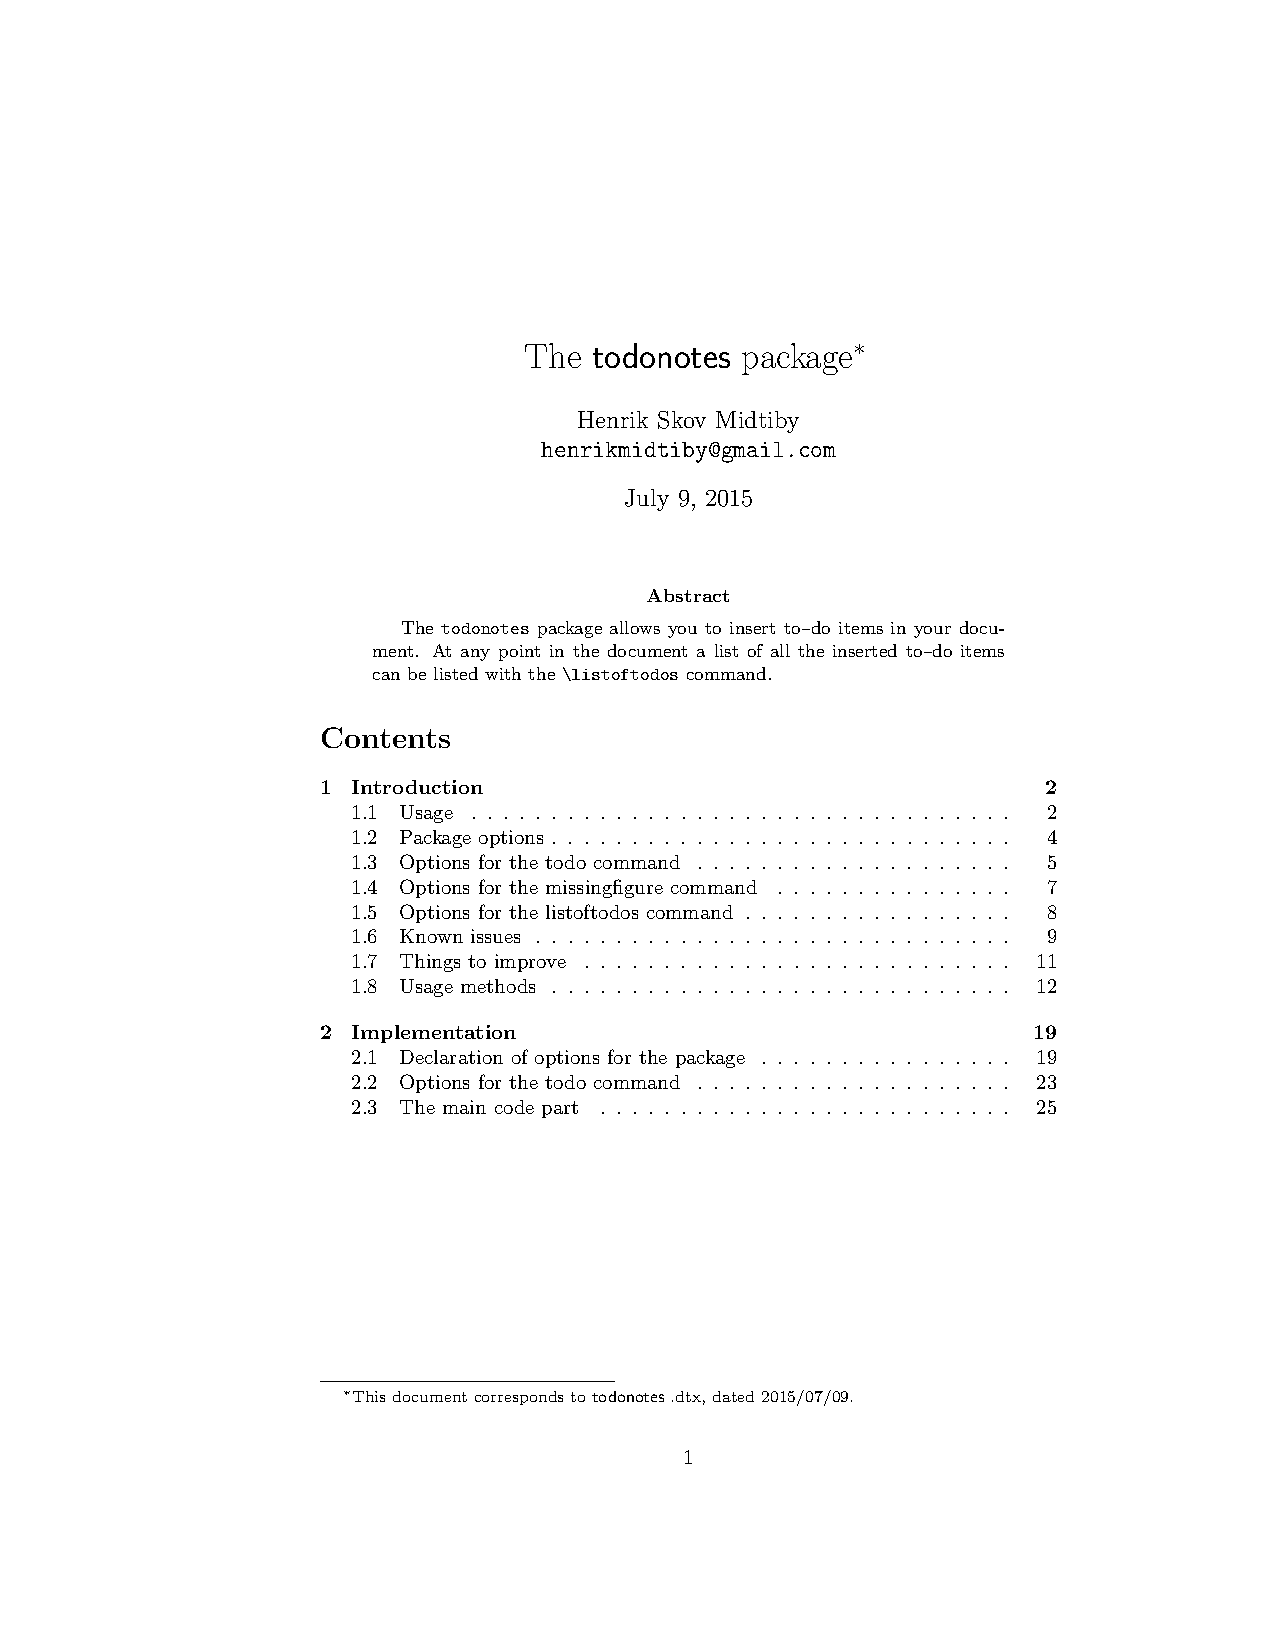
\includepdf[pages=1-3,scale=0.8,frame=true,pagecommand={}]{anexos/todonotes.pdf}
	
	
	% ---
	% Para incluir sem gerar a quebra de página inicial no anexo
	\chapter{Publicações no Blog}
	
	Esse apêndice trás os posts do blog semanal para demonstrar o desenvolvimento do projeto ao decorrer da matéria. 
	
	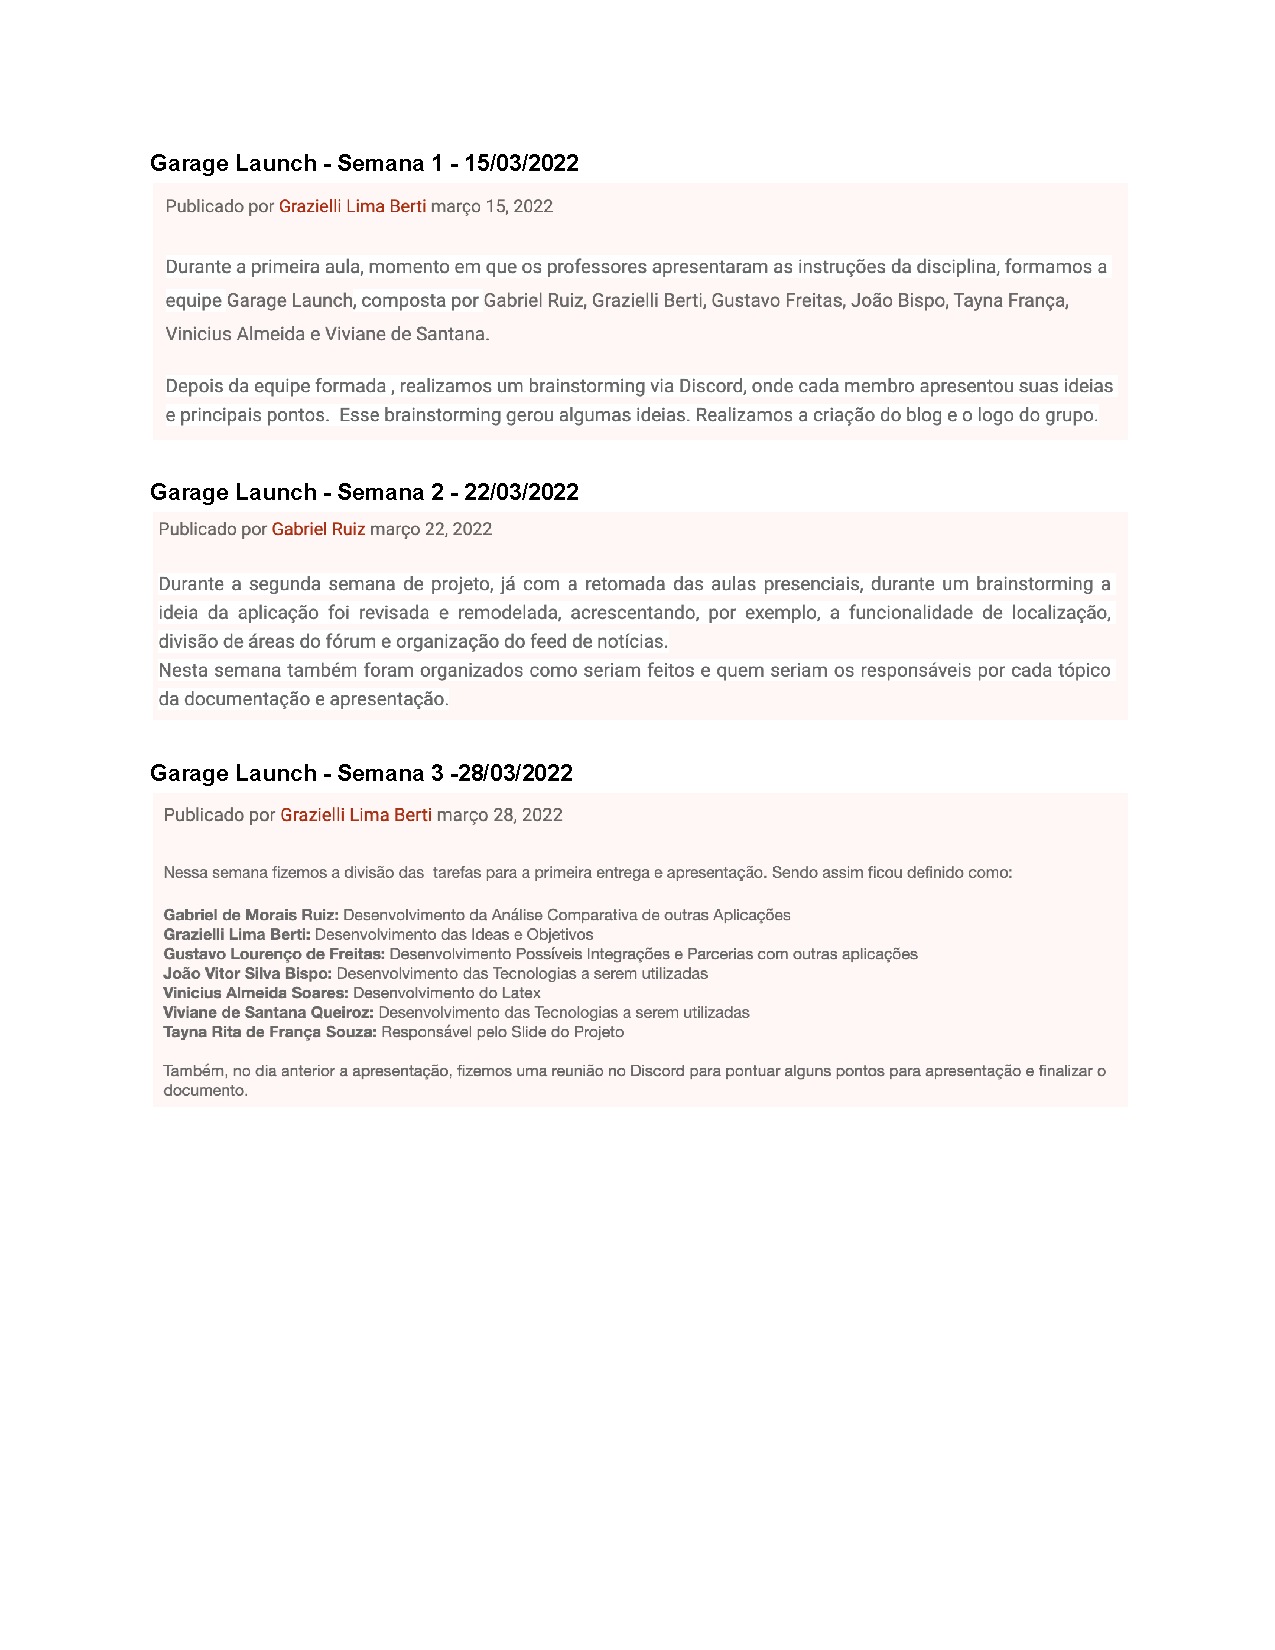
\includepdf[pages=1-6,scale=0.8,frame=true,pagecommand={}\label{publicacao-blog}]{anexos/Anexos_Todos_Os_Post_Do_Blog.pdf}
	
	
\end{apendicesenv}
% ---
